\documentclass[tikz, border=5pt]{standalone}
\usepackage{amsmath, bm, amssymb}
\usetikzlibrary{arrows.meta, positioning}

\newcommand{\R}{\mathbb{R}} % Defining your Real numbers symbol

\begin{document}
	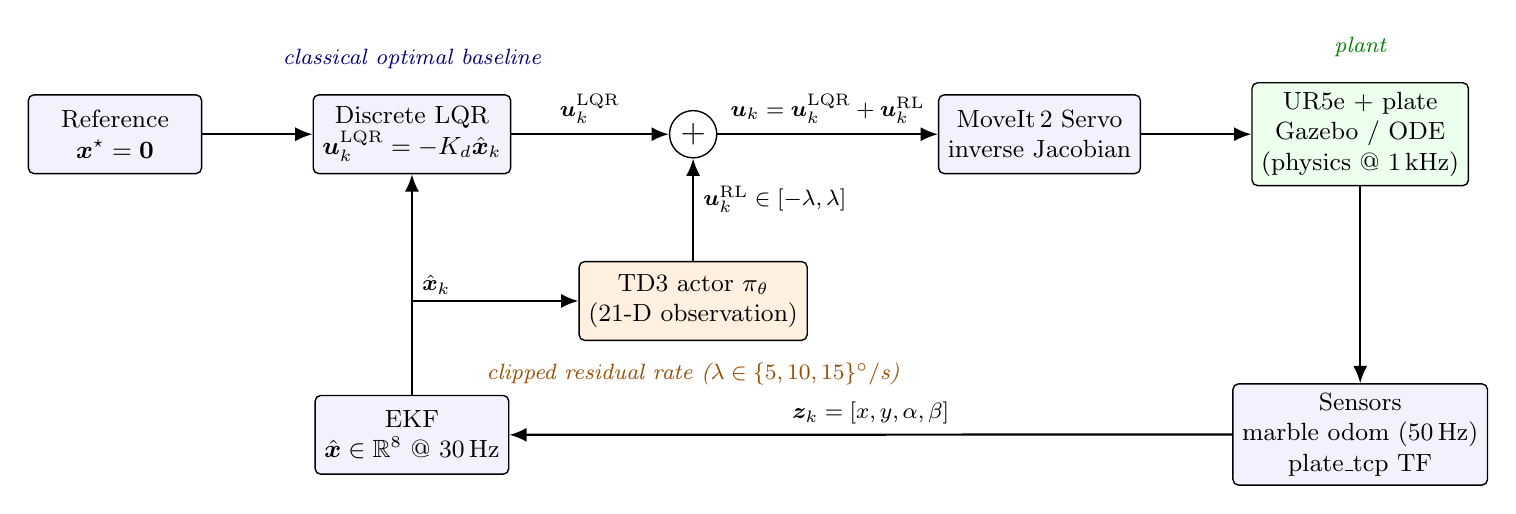
\begin{tikzpicture}[
		>={Latex[length=2.2mm,width=1.8mm]},
		every node/.style={font=\small},
		block/.style={draw, rectangle, rounded corners=2pt, minimum height=10mm, minimum width=22mm, align=center, fill=blue!5, line width=0.5pt},
		rl/.style={draw, rectangle, rounded corners=2pt, minimum height=10mm, minimum width=22mm, align=center, fill=orange!12, line width=0.5pt},
		plant/.style={draw, rectangle, rounded corners=2pt, minimum height=10mm, minimum width=24mm, align=center, fill=green!7, line width=0.5pt},
		sum/.style={draw, circle, minimum size=6mm, inner sep=0pt, fill=white, line width=0.5pt},
		sig/.style={font=\footnotesize}
		]
		
		% --- Top row: signal flow forward ---
		\node[block] (ref) {Reference\\$\bm{x}^\star=\bm{0}$};
		\node[block, right=14mm of ref] (lqr) {Discrete LQR\\$\bm{u}^{\text{LQR}}_k=-K_d\hat{\bm{x}}_k$};
		\node[sum, right=20mm of lqr] (sum) {\large$+$};
		\node[block, right=28mm of sum] (servo) {MoveIt\,2 Servo\\inverse Jacobian};
		\node[plant, right=14mm of servo] (ur5e) {UR5e $+$ plate\\Gazebo $/$ ODE\\(physics @ 1\,kHz)};
		
		% --- Bottom row: estimation + RL ---
		\node[block, below=28mm of lqr] (ekf) {EKF\\$\hat{\bm{x}}\in\R^8$ @ 30\,Hz};
		\node[block, below=25mm of ur5e] (sense) {Sensors\\marble odom (50\,Hz)\\plate\_tcp TF};
		\node[rl, below=13mm of sum] (td3) {TD3 actor $\pi_\theta$\\(21-D observation)};
		
		% --- Forward edges ---
		\draw[->, thick] (ref) -- (lqr);
		\draw[->, thick] (lqr) -- node[sig, above]{$\bm{u}^{\text{LQR}}_k$} (sum);
		\draw[->, thick] (sum) -- node[sig, above]{$\bm{u}_k=\bm{u}^{\text{LQR}}_k+\bm{u}^{\text{RL}}_k$} (servo);
		\draw[->, thick] (servo) -- (ur5e);
		
		% --- Sensor / EKF edges (no overlap) ---
		\draw[->, thick] (ur5e.south) -- (sense.north);
		\draw[->, thick] (sense.west) -- node[sig, above]{$\bm{z}_k=[x,y,\alpha,\beta]$} (ekf.east);
		\draw[->, thick] (ekf.north) -- node[sig, right]{$\hat{\bm{x}}_k$} (lqr.south);
		
		% --- EKF feeds residual observation (routed below ekf, then up into td3 from the left) ---
		\draw[->, thick] (ekf.north) -- ++(0.0,0) |- (td3.west);
		
		% --- TD3 output up into the sum ---
		\draw[->, thick] (td3.north) -- node[sig, right, pos=0.6]{$\bm{u}^{\text{RL}}_k\in[-\lambda,\lambda]$} (sum.south);
		
		% --- Region annotations ---
		\node[draw=none, font=\footnotesize\itshape, blue!50!black, above=2mm of lqr] {classical optimal baseline};
		\node[draw=none, font=\footnotesize\itshape, orange!60!black, below=1.5mm of td3] {clipped residual rate ($\lambda \in \{5,10,15\}^\circ/$s)};
		\node[draw=none, font=\footnotesize\itshape, green!50!black, above=2mm of ur5e] {plant};
	\end{tikzpicture}
\end{document}